% =============================================================================
\section{Applications}
\label{sec:app}
% =============================================================================
The \cgal{} library, and in particular the \cgal{} arrangement packages have been used intensively at the Computational Geometry Lab at Tel Aviv University for over twenty years now, not only for research, where the researchers typically
% (though not always)
(though not always---see Section~\ref{ssec:neural})
have good knowledge of generic programming in C++, but also for teaching. We have been using
%(in particular the third author of the paper)
\cgal{} for projects in the Computational Geometry course, for assignments and final projects in the courses ``Algorithmic Robotics and Motion Planning'' and ''Algorithms for 3D printing and other Manufacturing Processes'', and for the implementation of a variety of robot algorithms in guided software workshops. Using \cgal{} for teaching  has persistently been a pain-point in these courses especially due to the intricate  utilization of C++ in the implementation of the library. This has recently dramatically changed with the introduction of the Python bindings presented in this paper,
as we describe in two examples below.
% as we describe below.

%\begin{comment}
% -----------------------------------------------------------------------------
\subsection{A Multi Robot Motion Planning Platform}
\label{ssec:discopygal}
% -----------------------------------------------------------------------------
%\end{comment}
\begin{comment}
We were invited to give a crash course in multi-robot motion planning in a summer school geared primarily toward engineering doctoral students,\footnote{\url{http://disc.tudelft.nl/education/summer-school/disc-summer-school-2021/}} where the organizers particularly asked for hands-on algorithm implementation and experimentation session. For that we developed \disco{}, which is a program written in Python that provides visualization and verification for multi-robot motion planning in 2D.
% The program uses a subset of the Python bindings of \cgal{} (namely, \cgal{} arrangements, \cgal{} Minkowski sums, and other components of \cgal{} needed for the implementation of fundamental motion-planning algorithms),
The program uses Python bindings of \cgal{} arrangements, \cgal{} Minkowski sums, and other components of \cgal{} needed for the implementation of fundamental motion-planning algorithms,
and enables the dynamic loading of motion-planning algorithms in the form of Python scripts during run time. It allows users to easily swap and compare between different motion-planning algorithms, and even modify an existing implementation of an algorithm while the program is running. (There is no need to recompile the code or restart the program.) The precompiled library for the \cgal{} bindings used by the program is supplied with it, such that even the installation of \cgal{}, boost, or a C++ compiler is not required in order to use the program.
%
Eventually, in the course, after two hours of lecture including fifteen minutes of presentation of the software system, students installed it and were able to add new algorithms or modify and improve existing algorithms. Testimonies of students and organizers affirmed that the system was friendly and easy-to-use, and fruitful in assisting the students to absorb the algorithmic ideas. The students only needed to access and write Python code, while still employing heavy-duty \cgal{} procedures in the background.
\end{comment}
We developed a program called \disco{} written in Python that provides visualization and verification for multi-robot motion planning in 2D.  The program uses Python bindings of \cgal{} arrangements, \cgal{} Minkowski sums, and other components of \cgal{} needed for the implementation of fundamental motion-planning algorithms and enables the dynamic loading of motion-planning algorithms in the form of Python scripts during run time. It allows users to easily swap and compare between different motion-planning algorithms, and even modify an existing implementation of an algorithm while the program is running. (There is no need to recompile the code or restart the program.) The precompiled library for the \cgal{} bindings used by the program can be supplied with it, such that even the installation of \cgal{}, boost, or a C++ compiler is not required in order to use the program. We were invited to give a crash course in multi-robot motion planning in a summer school geared primarily toward engineering doctoral students,\footnote{\url{http://disc.tudelft.nl/education/summer-school/disc-summer-school-2021/}} where the organizers particularly asked for hands-on algorithm implementation and experimentation session. After two hours of lecture including fifteen minutes of presentation of \disco, students installed it and were able to interact with it. Testimonies of students and organizers affirmed that the system was friendly and easy-to-use, and fruitful in assisting the students to absorb the algorithmic ideas. The students only needed to access and write Python code, while still employing heavy-duty \cgal{} procedures in the background.

In this year's Algorithmic Robotics course, the experimental assignments are based on \disco{}. This is the first time that the introduction of the software into the assignment passed completely smoothly, without compromising the required level of algorithmic sophistication. The system allows the students to focus on algorithmic issues using Python, a programming language they are all familiar with, freeing them from many of the past points of hardship raised by working directly with \cgal{}, and in particular with the advanced generic-programming mechanisms that \cgal{} uses.

A snapshot of the \disco{} application window is shown in Figure~\ref{fig:disco}. The window is divided into three parts; informative messages are displayed on the console on the left, a rich menu resides to the right of the console; the workspace is drawn on the right. The particular workspace in the figure consists of two disc robots. The objective is to swap their positions. The path of each robot planned by the system is drawn in the color of the robot.

\begin{figure}[!htp]
  \centering%
  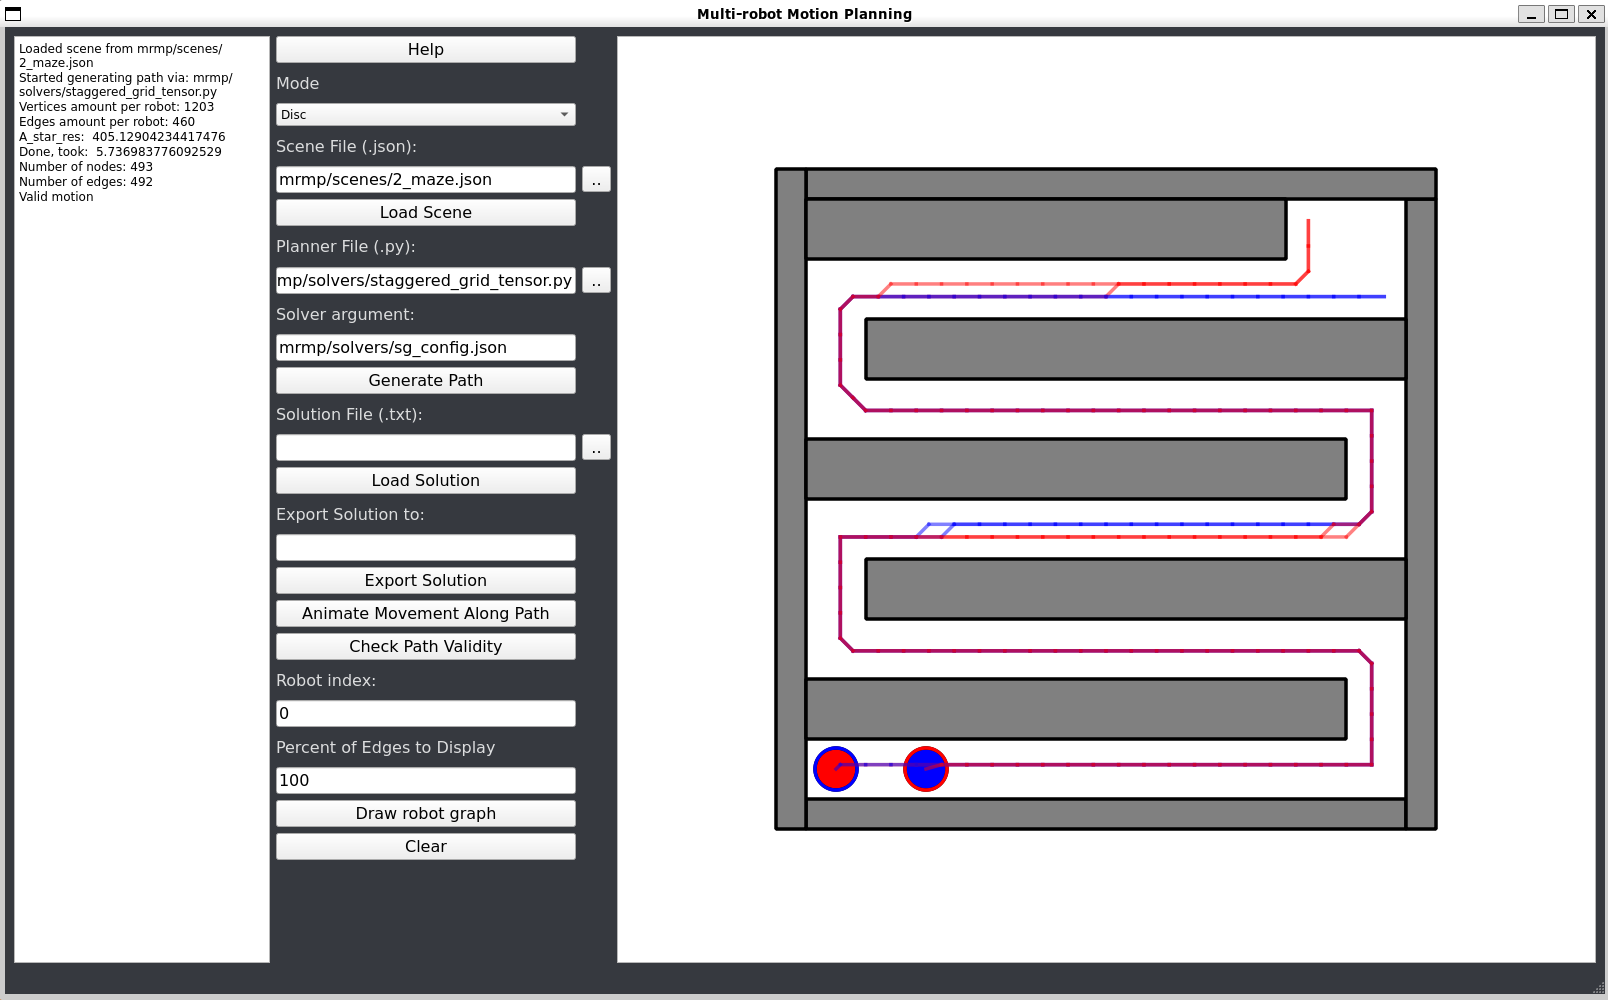
\includegraphics[width=\linewidth]{../figs/discoPygal_two_robots.png}
  \caption{A snapshot of the \disco{} application window.}
  \label{fig:disco}
\end{figure}

% -----------------------------------------------------------------------------
\subsection{Neural Collision Detection}
\label{ssec:neural}
% -----------------------------------------------------------------------------
% In collaboration with neuroscientists, we developed a simulation system for the interaction between neurons and blood vessels in the brain~\cite{Har-Gil2021.07.20.452894}. The need arose to use three-dimensional alpha shapes. The \cgal{} offerings in this respect looked a perfect fit, with the caveat that the main tools of the simulation are developed in Python and the most convenient programming language for that part of the project is Python. We developed Python bindings for the \cgal{} alpha-shape package, and their usage was immediately and almost effortlessly integrated into the overall system by the neuroscientists.
In collaboration with neuroscientists, we helped developing a simulation system that uses three-dimensional alpha shapes, for the interaction between neurons and blood vessels in the brain~\cite{Har-Gil2021.07.20.452894}. The \cgal{} offerings in this respect looked a perfect fit, with the caveat that the simulation was developed in Python, which is the most convenient programming language for the project. We developed Python bindings for the \cgal{} alpha-shape package, and their usage was almost effortlessly integrated into the system by the neuroscientists.
